% !TeX root = hauptprojekt.tex
% !TeX spellcheck = en_US

\documentclass[
,paper=a4
,twoside=false
,fontsize=11pt
,headsepline
,BCOR10mm
,DIV11
]{scrbook}
\usepackage[english, ngerman]{babel}
%% see http://www.tex.ac.uk/cgi-bin/texfaq2html?label=uselmfonts

% define \mysharp using the arev package
\usepackage{arev}
\newsavebox{\sharpbox}
\sbox{\sharpbox}{$\sharp$}
\newcommand{\mysharp}{\usebox{\sharpbox}}

\usepackage[T1]{fontenc}
\usepackage[utf8]{inputenc}
\usepackage{libertine}
\usepackage{pifont}
\usepackage{microtype}
\usepackage{textcomp}
\usepackage[english,refpage]{nomencl}
\usepackage{setspace}
\usepackage{makeidx}
\usepackage{listings}
\usepackage{natbib}
\usepackage[english,colorlinks=true]{hyperref}
\usepackage{soul}
\usepackage{hawstyle}
\usepackage{float}
\usepackage{csquotes}
\usepackage{tabularx}
\usepackage{subcaption}
\usepackage{usecases}
\usepackage{enumitem}
\usepackage{pgfplots}
\usepackage{siunitx}
\usepackage{lscape}


% Initializing the functional requirements
\newcommand{\reqinitF}{
	% Create a new counter for keeping track of the last number
	\newcounter{reqcountbackupF}
	% Create a new counter for the custom label
	\newcounter{reqcountF}
	% Redefine the command for the last counter so when it is called
	% it prints the number like this in a bold font: R<number>
	\renewcommand{\thereqcountF}{\textbf{F\arabic{reqcountF}}}
}

% Used to define the start of the requirements
\newcommand{\reqstartF}{
	% Indicate the start of a new list and tell it to use the redefined
	% command and corresponding counter for every item
	\begin{list}{\thereqcountF}{\usecounter{reqcountF}}
		% Important part: set the value of the used counter to the
		% same value of the backup counter.
		\setcounter{reqcountF}{\value{reqcountbackupF}}
	}
	
	% Used to define the end of the requirements
	\newcommand{\reqendF}{
		% Important part: take the value of the used counter (after
		% being incremented by the requirement items) and store it
		% in the backup counter.
		\setcounter{reqcountbackupF}{\value{reqcountF}}
		% Mark the end of the list environment
	\end{list}
}

% Initializing the non-functional requirements
\newcommand{\reqinitNF}{
	\newcounter{reqcountbackupNF}
	\newcounter{reqcountNF}
	\renewcommand{\thereqcountNF}{\textbf{NF\arabic{reqcountNF}}}
}

\newcommand{\reqstartNF}{
	\begin{list}{\thereqcountNF}{\usecounter{reqcountNF}}
		\setcounter{reqcountNF}{\value{reqcountbackupNF}}
	}
	
	\newcommand{\reqendNF}{
		\setcounter{reqcountbackupNF}{\value{reqcountNF}}
	\end{list}
}

%% define some colors
\colorlet{BackgroundColor}{gray!20}
\colorlet{KeywordColor}{blue}
\colorlet{CommentColor}{black!60}
%% for tables
\colorlet{HeadColor}{gray!60}
\colorlet{Color1}{blue!10}
\colorlet{Color2}{white}

%% configure colors
\HAWifprinter{
	\colorlet{BackgroundColor}{gray!20}
	\colorlet{KeywordColor}{black}
	\colorlet{CommentColor}{gray}
	% for tables
	\colorlet{HeadColor}{gray!60}
	\colorlet{Color1}{gray!40}
	\colorlet{Color2}{white}
}{}
\lstset{%
	numbers=left,
	numberstyle=\tiny,
	stepnumber=1,
	numbersep=5pt,
	basicstyle=\ttfamily\small,
	keywordstyle=\color{KeywordColor}\bfseries,
	identifierstyle=\color{black},
	commentstyle=\color{CommentColor},
	backgroundcolor=\color{BackgroundColor},
	captionpos=b,
	fontadjust=true
}
\lstset{escapeinside={(*@}{@*)}, % used to enter latex code inside listings
	morekeywords={uint32_t, int32_t}
}
\ifpdfoutput{
	\hypersetup{bookmarksopen=false,bookmarksnumbered,linktocpage}
}{}

\clubpenalty=10000
\widowpenalty=10000
\displaywidowpenalty=10000

% unknown hyphenations
%\hyphenation{
%}

%% recalculate text area
\typearea[current]{last}

\makeindex
\makenomenclature

\begin{document}
	\selectlanguage{english}
	
	
	%%%%%
	%% customize (see readme.pdf for supported values)
	\HAWThesisProperties{Author={Lennart Karsten}
		,Title={Optimizing geospatial read-performance\\inside a multi-agent simulation system}
%		,EnglishTitle={Optimizing geospatial read-performance inside a multi-agent simulation system}
		,ThesisType={Hauptprojekt}
		,ExaminationType={Masterprüfung}
		,DegreeProgramme={Master Informatik}
		,ThesisExperts={Prof. Dr. Thomas Clemen}
		,ReleaseDate={\today}
	}

	%% title
	\frontmatter
	
	%% output title page
	\maketitle
	
	\onehalfspacing
	
	%% add abstract pages
	%% note: this is one command on multiple lines
	\HAWAbstractPage
	%% German abstract
	{GIS, performance, Multi-agent simulation}%
	{This work evaluates and suggests improvements to the geospatial performance of a multi-agent simulation system. The suggestions are evaluated and performance tested and the results allow GIS to be used for large scale simulations.\\}
	%% English abstract
%	{GIS, performance, Multi-agent simulation}%
%	{english abstract.}
	
	\newpage
	\singlespacing
	
	\tableofcontents
	\newpage
	%% enable if these lists should be shown on their own page
	%\listoftables
	%\listoffigures
	%\lstlistoflistings
	
	%% main
	\mainmatter
	\onehalfspacing
	% write to the log/stdout
	\typeout{===== File: chapter 1}

	% init requirements	
	\reqinitF
	\reqinitNF

	% !TeX spellcheck = en_US

\chapter{Introduction}
Geo-spatial data plays a major roll in the processing big data and in the ages of mobile geo-referenced data is becoming increasingly relevant \citep{Lee2015, Kitchin2013, Graham2013}. With growing relevance of such big data, the efficient storage and manipulation is a crucial topic.\\
MARS LIFE provides a large scale simulation environment for multi-agent simulations. Most models rely on geo-referenced data, making it a natural match for GIS. The possibility to use it as input for simulations is therefor very desirable.\\
This work focuses on improving the LIFE simulation system by adding layers that allows to take advantage of raster and vector GIS capabilities.



\section{Motivation}
MARS LIFE used to have capabilities for using GIS. However, they did not meet the requirements in terms of performance and usability. For this reason they were never used in production. With a recent infrastructural change, it has been abandoned due to incompatibilities.\\
The incapability to use GIS created the necessary for workarounds to use geo-referenced data. While these solutions work, they cover a very narrow use-case tailored to the needs of a specific model. This contradicts the idea of a general purpose simulation system.\\
For the reasons mentioned above this work focuses on re-instantiating the GIS into MARS LIFE and to meet the requirements in terms of performance and usability. The main focus is, to achieve a performance that can handle agent counts in the millions within a reasonable time.
 % Introduction
	% !TeX spellcheck = en_US

% GIS Grundlagen
% GIS Libs & Software
% Datenbanken
% MARS Architektur + Rahmenbedingungen
\chapter{Basics}
This chapter elaborates on the fundamental concepts and technologies necessary to understand the following chapters. They consist of a general overview of Geographic Information Systems, the mentioned geospatial libraries and databases, as well as the MARS Eco-System and it's environment.



\section{Geographic Information System (GIS)}
GIS consists of numerous technologies to store, manipulate, analyze and visualize geographical data. It can be used in all domains that require the use of temporal and spatial data. Some usages are the visualization of land-use, elevation data, weather maps, street networks and flood maps. To leverage the capabilities that GIS offers, specialized software is required that can handle the spatial references, such as ESRI ArcMap, QGIS or GrassGIS.


\subsection{Coordinate Reference System (CRS)}
In comparison to normal image data, such as JPEG or PNG, GIS data is geo-referenced, meaning each feature or pixel has a geospatial location. This is achieved by specific geo-aware formats that encode spatial positions into the data. This location is represented in a coordinate system. In GIS terminology this is referred to as \enquote{spatial reference system} (SRS) or \enquote{coordinate reference system} (CRS). Depending on the spatial area, coordinate systems provide different accuracy in their results. Some are optimized for certain areas, while others offer a general worldwide accuracy. The following sections explain common reference systems.

\subsubsection{Mercator Projection}
The most globally used CRS is the Mercator projection. I was created by Gerardus Mercator in 1569 \cite{meer2012atlas} and has been improved over the years. Figure \ref{fig:mercator} shows the Mercator projection in it's normal (left) and transverse (right) orientation. The normal projection offers good general representation, while the transverse orientation is focuses on the poles.
\begin{figure}[H]
	\centering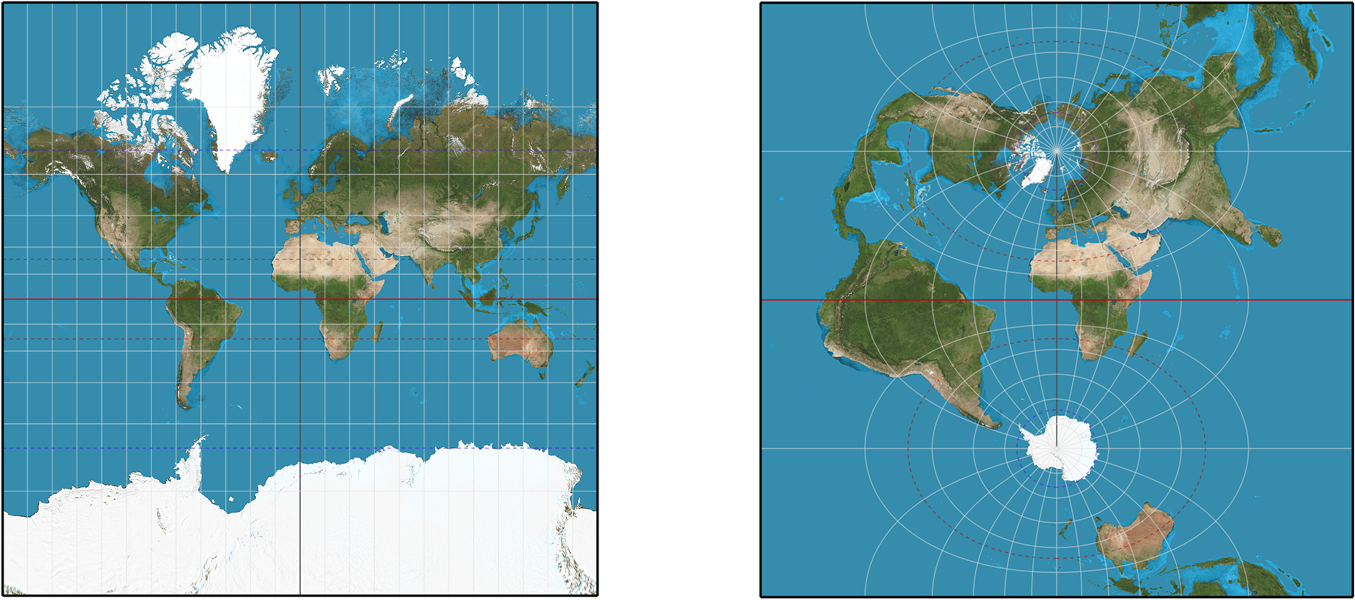
\includegraphics[width=1\textwidth]{res/Mercator}
	\caption{Normal and transverse Mercator projection. \url{https://commons.wikimedia.org/w/index.php?curid=9910866}}
	\label{fig:mercator}
\end{figure}

\subsubsection{EPSG:4326 -- WGS 84}
The most recent version of the Mercator projection is called WGS 84. It improves in accuracy compared to WGS 72 and is an \enquote{European Petroleum Survey Group} (EPSG) standard called EPSG:4326, created by \cite{Decker1986}.\\
WGS 84 is an ellipsoidal coordinate system that shows the 3D surface of the earth in 2D. The coordinates are longitude and latitude measured in degree. Longitude has the 0° point in Greenwich, England and increases east to a maximum of 180° and west to a minimum of -180°. Latitude has the 0° point at the equator and increases north to a maximum of 90° and south to a minimum of -90.\\
WGS 84 is used by the Global Positioning System (GPS), GIS specialists, inside the OpenStreetMap (OSM) database, as well as Google Earth.

\subsubsection{EPSG:3857 -- WGS 84 / Pseudo-Mercator}
Pseudo-Mercator is a projected version of WGS 84 into a two-dimensional cartesian coordinate system. It is also referred to as EPSG:3857 and was created by \cite{Grafarend1995}.\\
The CRS is based on a plane, rather than an ellipse. The zero points is identical to WGS 84 but the coordinates are X and Y measured in meters. The Y coordinate is limited to ±85.06° of the WGS 84 bounds. This results in a square projection with a range of ±20,026,376.39m on both axis, but sacrifices the poles to some extend. The square shape allow the creation of tile pyramids, also called \enquote{Mercator Pyramids} to be used for maps in browsers for the web.\\
A pyramid consists of square images in fixed size, e.g. 256x256px. The First level has one image that shows the whole area of the data with minimal detail. On every level below the number of image tiles increases and therefore the level of detail. The number of tiles on a given level is
$$x_n= 4* x_{n-1}$$ 
where \enquote{x} is the number of tiles and \enquote{n} is the current level of detail. Figure \ref{img:mercator-pyramid} shows an example of a Mercator pyramid.
\begin{figure}[H]
	\centering
	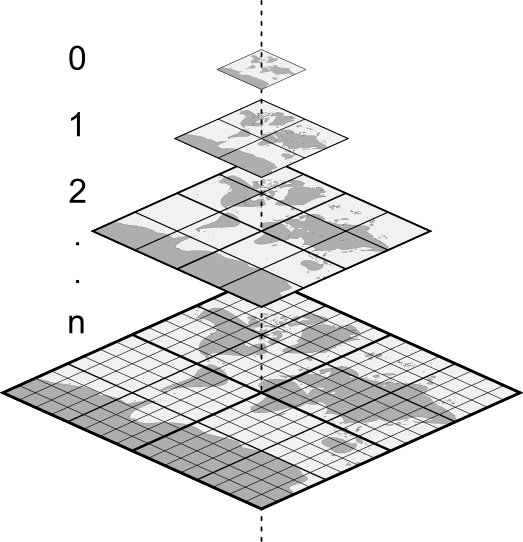
\includegraphics[width=0.4\columnwidth]{res/mercator-pyramid}\\
	\caption[]{Mercator tile pyramid. \url{http://data.webglearth.com/doc/webgl-earthch1.html}}
	\label{img:mercator-pyramid}
\end{figure}
This fragmentation of a big dataset is optimal to be loaded on demand and cached by a web browser, which is why major map sites, like OpenStreetMap, Google Maps and Bing Maps use Pseudo-Mercator as their reference system.


\subsection{Spatial Data Types}
Geo-spatial data exist in two different types, vector and raster. 

\subsubsection{Raster Data}
 Raster data consists of a grid in fixed size. Depending on the file, each pixel contains a color (e.g. satellite data)  or a grayscale (e.g. elevation maps) value.\\
 The advantage of raster data is that it is better suited to store picture like data with gradients. Due to its nature, raster has data in every cell, which leads into a high amount of data that has to be stored, so the potential file size if big.\\
 Since the raster size is fixed, the balance between desired detail and small file size has to be decided upon file creation. Figure \ref{img:raster} shows a shape in three different rasterized resolutions, visualizing the loss of detail.
 \begin{figure}[H]
 	\centering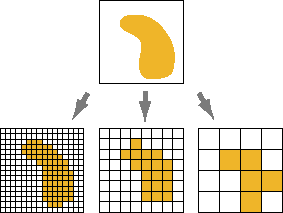
\includegraphics[width=.5\textwidth]{res/Vector-Raster}
 	\caption{Shape as raster in different resolutions. \url{http://desktop.arcgis.com/en/arcmap/latest/manage-data/raster-and-images/what-is-raster-data.htm}}
 	\label{img:raster}
 \end{figure}
Common file types for raster data are GeoTIFF, ESRI, ESRI ArcGrid and ASCIIGrid. GeoTIFF and ArcGrid are binary file types and ASCIIGrid is text-based.

\subsubsection{Vector Data}
In contrary to raster data, vectors files don't map color information to a specific pixel, but define mathematical shapes which are rendered as desired. This allows very efficient storage and it is possible to scale the shapes as desired.\\
Data inside vector GIS can have several layers. Each layer has the type points, line or polygon. The data on a layer is called a feature and matches the layer's type. A point feature has a single coordinate (e.g. a well in the ground). Lines are open polygon lines and are used for shapes like walls, streets or rivers. Polygons are closed lines and are used for areas, such as countries, lakes, or larger objects. Figure \ref{img:vector} shows a vector file with the mentioned 3 layers types. The point layer shows the position of wells, the line layer shows a river and the polygon layer a lake.\\
While vector files have the advantage of efficient storage, they have the disadvantage of not being universally usable. The mathematical functions in which data is represented, are not well suited for data without discrete values. Anything that has gradients is better suited for raster.\\
The most common vector file formats are ESRI Shapefile as binary and GeoJSON as a text-based format.

\begin{figure}[H]
	\centering
	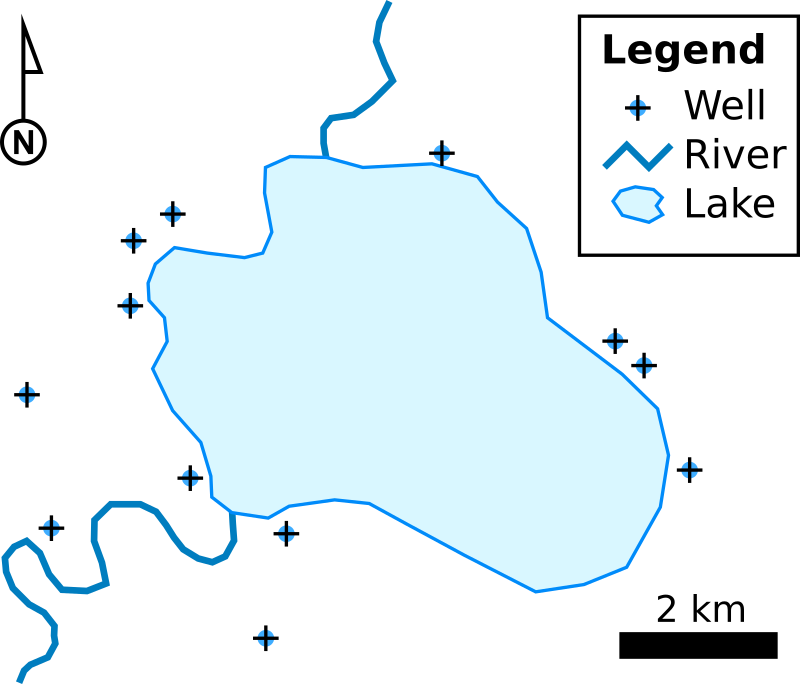
\includegraphics[width=0.4\columnwidth]{res/vector-map}\\
	\caption[]{Vector map with point, line and polygon. \url{https://commons.wikimedia.org/w/index.php?curid=3024482}}
	\label{img:vector}
\end{figure}



\section{GIS Technologies}
This chapter introduces the GIS technologies that were considered for usage during this work. They are grouped into \enquote{spatial databases}, \enquote{GIS Libraries} and \enquote{Others}. Figure \ref{fig:technology_overview} shows a brief overview and compatibility of the libraries.

\begin{table}[H]
	\caption{GIS solutions feature comparison}
	\label{fig:technology_overview}
	\begin{tabular}{|l|l|l|l|}
		\hline \textbf{Name}	& \textbf{Raster support} & \textbf{Vector support} & \textbf{Type}\\
		\hline PostGIS	& Yes* & Yes & PostgreSQL DB + GIS ext.\\
		\hline MongoDB	& No & Yes & NoSQL DB with spatial capabilities\\\hline
		\hline Dotspatial & Yes & Yes & C\# library\\
		\hline NetTopologySuite	& No & Yes & C\# library\\\hline
		\hline GeoServer & Yes & Yes & Self-hosted product\\
		\hline GDAL & Yes & Yes & Library for geospatial manipulation\\
		\hline
	\end{tabular}
	\caption*{ \raggedright * Large file failed.}
\end{table}


\subsection{Spatial Databases}
Spatial databases are DBs that have been extended to store and query spatial data types.

\subsubsection{PostGIS}
PostGIS is an extender to the object-relational database PostgreSQL that allows to store and query both raster and vector GIS. The interaction with the database is done through SQL.\\
PostGIS supports numerous file types for both raster and vector data. The import process is done with specific tools that come as command-line applications which are bundled into the installation. The geometry type allows spatial queries regarding certain areas. These allow to extract single pixel values from raster files as well as feature extraction from vector files.\\
To read more about PostGIS and PostgreSQL see \cite{Obe2011} and \cite{Momjian2001}.

\subsubsection{MongoDB}
MongoDB is a document-based (NoSQL) database. Data is stored in binary JSON (BSON) and input, as well as output data is in JSON format.\\
As of version 3.4.9 MongoDB supports only vector GIS. It does not support a wide range of format types, but only GeoJSON \citep{Butler2016}. However, it is quite easy to convert the common vector files to GeoJSON using GDAL (see \ref{sec:gdal} for more details).


\subsection{GIS Libraries}
The amount of proper maintained GIS libraries for C\# is very limited. DotSpatial and NetTopologySuite are among the only libraries with at least community support behind them.

\subsubsection{DotSpatial}
DotSpatial is a GIS library for .Net Framework that allows reading and writing both raster and vector data. Besides it's manipulation capabilities, it offers functionality for map visualization that allows displaying data. Unfortunately the library has not been ported to .Net Core yet.

\subsubsection{NetTopologySuite (NTS)}
NetTopologySuite is a C\# reimplementation of the JTS Topology Suite (formerly known as "Java Topology Suite"). It is a library for geospatial vector data manipulation. Raster data handling is not supported. The Library has been migrated to support .NET Core in the fall of 2017.

\subsubsection{AsciiGridParser}
Since DotSpatial is not ported to .NET Core yet, there is no acceptable solution for reading raster GIS during the simulation. This is, why the author of this work created a parser for Esri's ASCII grid format.\\
ASCII grid is a text-based, geo-referenced raster format that other raster formats like GeoTIFF can be converted into.


\subsection{Others}
The following technologies did not fit the previous categories. The GeoServer stores and manages GIS yet is not database itself and GDAL is a GIS library which is used as standalone software.

\subsubsection{GeoServer} \label{sec:GS}
The GeoServer is an open source software that is tailored to store, manage and share GIS. It offers a web UI as well as a REST API for interaction. The API is structured in a way that it implements common Open Geospatial Consortium (OGC) standards for retrieving data.\\
The Web Feature Service (WFS) allows to retrieve features of vector data, Web Coverage Service (WCS) enables downloading raster data and the Web Map Service (WMS) can generate a tile map for viewing GIS on a map.
%\\The GeoServer is build for working with few files and a small number of users. The MARS use-case requires to read thousands to millions of single values in parallel in a short amount of time. The GeoServer does not satisfy this demands. The retrieval of single values is not supported, since the general use-case is to work with complete files and the performance for retrieving data is very poor which will require a better solution.\\
%figure \ref{img:gs-read-performance} emphasizes this. It shows GeoServer response time for different storage solutions. All values exceed one second which is not expectable for the amount of requests needed for this work. \cite{Pandey2016} argues that disk-based systems are generally not fast enough for real-time analysis.
%
%\begin{figure}[H]
%	\centering
%	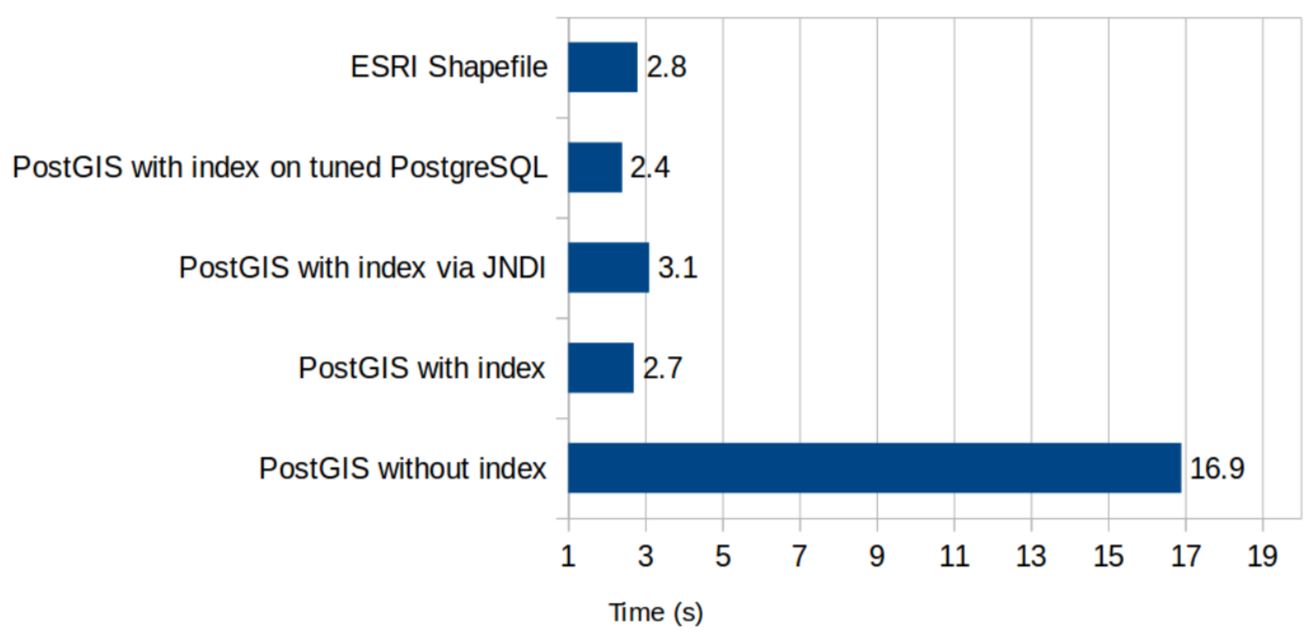
\includegraphics[width=0.8\columnwidth]{res/gs-read-performance}\\
%	\caption[]{GeoServer average time of response by \cite{ruuvzivcka2016comparing}}
%	\label{img:gs-read-performance}
%\end{figure}

\subsubsection{Geospatial Data Abstraction Library (GDAL)}
\label{sec:gdal}
GDAL is a GIS library that is capable of reading and converting various data formats. It current version (2.2.2) supports 142 different raster and 84 vector formats. The library is distributed as a combination of various command-line tools that are each tailored at a specific task. E.g. gdal\_translate converts files between different formates.\\
The gdal tools work with raster data and the ogr tools work with vector data. Ogr stands for \enquote{OpenGIS Simple Features Reference Implementation} and is bundled in the gdal installation.


\section{MARS}
MARS (Multi-Agent Research and Simulation) is a working group at the HAW (University of applied Sciences) in Hamburg, Germany. The research group develops an distributed agent-based simulation system \citep{Wooldridge2009} to be used by domain experts around the world. It consists of several components.


\subsection{LIFE}
The simulation system is called MARS LIFE. It executes simulation. For more detail see \cite{Huning2016}.


\subsection{Cloud Services}
The Cloud Services are the central back-end of the MARS system. These components are responsible for data import, persistence, data visualization an the connection between LIFE and the WebUI.


\subsection{WebUI}
The WebUI is the front-end of MARS. It is a web-based application that allows the user to control back-end services and trigger simulations from the web-browser. The mentioned UI is not the one explained by \cite{Karsten2017}, but an alternative implementation.



\section{C\# Platforms}
The LIFE simulation system is written in the C\# language. There are however differences between the three platforms .NET Framework, Mono and .NET Core which are important for the implementation of this work.


\subsection{.NET Framework}
.NET Framework is the original platform C\# runs on. It is widely used in the industry and is supported by Microsoft. Unfortunately it only works in combination with Windows, which is why the community created Mono.

\subsection{Mono}
Mono is an open C\# implementation which is cross platform and therefore also available for Linux and OSX. The implementation of Mono is almost complete, which makes most applications that don't require platform specific code, like GUI modules, run on multiple platforms. The implementation of Mono is not build for high performance use-cases like MARS.

\subsection{.NET Core}
In 2016 Microsoft released it's own platform independent .NET version, called .NET Core. It is a complete rewrite of the .NET Framework to satisfy the shortcomings of both alternative solutions.\\
With it's current version (2.0) it has still some missing core functions, which leads to incompatibilities regarding existing software.
 % Basics
	% !TeX spellcheck = en_US

\chapter{Analysis}
The goal of this work is to create a layer inside the simulation system MARS LIFE that allows loading GIS in an high-performance way. To ensure the practical use to the model developers use-cases were taken into account to generate requirements for the implementation.



\section{Use-Cases}
\begin{usecase}
	\addtitle{Vector I}{Read all features}
	\addfield{Summary:}{Read features from vector files with the following types: 
		\begin{itemize}[itemsep=-.25em]
			\item Point
			\item Polyline
			\item Polygon
		\end{itemize}
	}
	\additemizedfield{Preconditions:}{
		\item The vector file was imported prior to the simulation run.
	}
	\additemizedfield{Primary Scenario:}{
		\item A layer wants to read the position of agents during the initialization.
	}
%	\additemizedfield{Alternative Scenario:}{
%		\item The user clicks the upload button, browses files of his local machine, fills the form for every file and starts the import.
%	}
\end{usecase}

\begin{usecase}
	\addtitle{Vector II}{Read feature at position}
	\addfield{Summary:}{Read the closest feature to a GPS position.
	}
	\additemizedfield{Preconditions:}{
		\item The vector file was imported prior to the simulation run.
	}
	\additemizedfield{Primary Scenario:}{
		\item An agent wants to find a point of interest in his area (e.g. An elephant looking for the closest waterhole).
	}
\end{usecase}

\begin{usecase}
	\addtitle{Vector III}{Calculate distance between features}
	\addfield{Summary:}{A function that takes two features of different types as input and returns the distance in meters.
	}
	\additemizedfield{Preconditions:}{
		\item Both features exist and are available to the layer.
	}
	\additemizedfield{Primary Scenario:}{
		\item An agent wants to know the distance to a specific pint of interest.
	}
\end{usecase}

\section{Requirements}


\subsection{Functional Requirements}
\reqstartF
	\item Point and area
	\item GPS position
	\item Determine distance to a feature (POI)
	\item Check if position overlaps with a polygon
	\item Follow polygon (e.g. rivers)
\reqendF


\subsection{Non-Functional Requirements}
%\reqstartNF
%\item 
%\reqendNF % Analysis
	% !TeX spellcheck = en_US

\chapter{Software Design}
This chapter discusses the possible solutions for working with GIS inside the LIFE simulation system.



\section{Current state}
Currently the GIS support inside MARS is partial, some components of the environment are capable of handling GIS, while others are not currently supporting it.


\subsection{Web browser Front-end}
The WebUI supports GIS for importing and managing this kind of data. It's successor the teaching UI currently does not support GIS. Due to the micro-service structure of the back-end services it is possible for the front-ends to coexist.

\subsection{Back-end Services}
The back-end services fully support GIS. The file service accepts the uploaded files and hands control over to the GIS Data Service (GDS). 

\subsubsection{GIS Data Service}
The GDS is capable of handling the most common GIS types, these are Geotiff and Esri AsciiGrid for raster and Shapefile for vector files. The files may be provided compressed inside a .zip file or as plain files.\\
During the import the GDS determines the type of data automatically by checking the file extension. Once detected, the file is validated and the spatial reference is determined. In case of a valid geo-referenced input, the file is imported into the GeoServer for persistence.


\subsubsection{GeoServer} \label{sec:GS}
The GeoServer (GS) is an open source software that is tailored to store, manage and share GIS. It offers a web GUI as well as a REST API for interaction. The api is structured in a way that it implements common Open Geospatial Consortium (OGC) standards for retrieving data.\\
The Web Feature Service (WFS) allows to retrieve features of vector data, Web Coverage Service (WCS) enables downloading raster data and the Web Map Service (WMS) can generate a tile map for viewing GIS on a map.\\
The GS is build for working with few files and a small number of users. The MARS use-case requires to read thousands to millions of  single values in parallel in a short amount of time. The GS does not satisfy this demands. The retrieval of single values is not supported, since the general use-case is to work with complete files. The performance for retrieving data is also very poor which will require a better solution.


\subsection{GIS Layer}
The GIS Layer inside MARS LIFE reads the Data provided by the GDS and uses it inside the simulation. Since the migration from C\# to .NET Core inside LIFE the GIS layer is not compatible anymore.\\
The current models therefore do not leverage GIS for their input. Data is being transfered into other formats to work around these shortcomings. Vector data is mainly represented as comma separated values (.csv) files and raster data are represented in custom formats.


\section{Solutions}
As mentioned in section \ref{sec:GS} reading data from the GS in real time is not feasible for a high performance environment.\\
Different alternative solutions have been discovered and evaluated. The files could be stored inside a spatial database (PostGIS or MongoDB) that is optimized for parallel reads of single values or the GIS file could be supplied to the Simulation and stored in memory for fast reading.

\begin{table}[]
	\centering
	\caption{My caption}
	\label{my-label}
	\begin{tabular}{|l|l|l|l|}
	\hline \textbf{Name}	& \textbf{Raster support} & \textbf{Vector support} & \textbf{Type} \\
	\hline GeoServer & yes & yes & self-hosted product \\
	\hline PostGIS	& yes* & yes & Database \\
	\hline MongoDB	& no & yes & Database \\
	\hline Dotspatial & yes & yes & C\# library \\
	\hline NetTopologySuite	& no & yes & C\# library \\
	\hline
	\end{tabular}
\end{table}

\subsection{PostGIS}
Large file: out of memory. Limit to 7 parallel threads solves it, but took 342,197ms

\subsection{MongoDB}


\subsection{Local library}



\section{Performance comparison}

\begin{tikzpicture}
\begin{axis}[
title  = Shapefile performance for 1k reads,
xbar,
y axis line style = { opacity = 0 },
axis x line       = bottom,
tickwidth         = 0pt,
%	enlarge y limits  = 0.02,
enlarge x limits  = 0.02,
symbolic y coords = {NetTopologySuite, DotSpatial, MongoDB, PostGis, Geoserver},
nodes near coords,
height=9cm,
legend style={at={(0.8,0.25)},anchor=north},
xlabel={Time in ms},
]
% Small Shapefile
\addplot coordinates {
	(23103,Geoserver)
	(160,PostGis)
	(135,MongoDB)
	(86,DotSpatial)
	(6,NetTopologySuite)
};
% Mid Shapefile
\addplot coordinates {
	(25307,Geoserver)
	(410,PostGis)
	(168,MongoDB)
	(251,DotSpatial)
	(193,NetTopologySuite)
};
% Large Shapefile
\addplot coordinates {
	(67727,Geoserver)
	(4789,PostGis)
	(223,MongoDB)
	(620,DotSpatial)
	(248,NetTopologySuite)
};
\legend{Small Shapefile (12 KB), Medium Shapefile (6.5 MB), Large Shapefile (103.8 MB)}
\end{axis}
\end{tikzpicture}

\begin{tikzpicture}
\begin{axis}[
title  = Raster performance for 1k reads,
xbar,
y axis line style = { opacity = 0 },
axis x line       = bottom,
tickwidth         = 0pt,
enlarge y limits  = 0.15,
enlarge x limits  = 0.02,
symbolic y coords = {DotSpatial, Local, PostGis, Geoserver},
nodes near coords,
legend style={at={(0.8,0.32)},anchor=north},
xlabel={Time in ms},
]
% Small Rasterfile
\addplot coordinates {
	(22202,Geoserver)
	(210,PostGis)
	(13,Local)
	(4,DotSpatial)
};
% Mid Rasterfile
\addplot coordinates {
	(24438,Geoserver)
	(1964,PostGis)
	(311,Local)
	(185,DotSpatial)
};
% Large Rasterfile
\addplot coordinates {
	(26786,Geoserver)
	(-1,PostGis) % 342197
	(273,DotSpatial)
	(467,Local)
};
\legend{Small raster (8 KB), Medium raster (6.4 MB), Large raster (105.2 MB)}
\end{axis}
\end{tikzpicture}
 % Software Design
	% !TeX spellcheck = en_US

\chapter{End}



\section{Conclusion}



\section{Outlook}
 % Implementation
	% !TeX spellcheck = en_US

\chapter{End}



\section{Conclusion}



\section{Outlook}
 % End
	
	%% appendix if used
	\appendix
	\typeout{===== File: appendix}
	% !TeX spellcheck = en_US

\begin{landscape}

\chapter{Appendix}

\begin{table}[H]
	\caption{GIS Technology overview}
	\label{fig:technologies}
	\resizebox{1.1\linewidth}{!}{
	\begin{tabular}{|l|l|l|l|}
		\hline \textbf{Name} & \textbf{Description} & \textbf{Discarded} & \textbf{URL}\\
		\hline AsciiGridParser & Own .NET Core Component & No & --\\
		\hline Dotspatial & C\# library & No & \url{https://github.com/DotSpatial/DotSpatial}\\
		\hline GeoServer & Self-hosted product & No & \url{http://geoserver.org}\\
		\hline MongoDB	& DB with spatial capabilities & No & \url{https://www.mongodb.com}\\
		\hline NetTopologySuite	& C\# library & No & \url{https://github.com/NetTopologySuite/NetTopologySuite}\\
		\hline PostGIS	& PostgreSQL DB + GIS ext. & No & \url{http://postgis.net}\\
		\hline
		\hline GeoMesa & Spatial-temporal database & Yes &  \cite{Toups2016}\\
		\hline HadoopDB & Hybrid of MapReduce and DBMS Technologies for Analytical Workloads. & Yes & \cite{Abouzeid2009}\\
		\hline Hadoop-GIS & A High Performance Spatial Data Warehousing System over MapReduce. & Yes & \cite{Wang2011}\\
		\hline Vertica & A proprietary analytic database owned by Hewlett Packard. & Yes & \url{https://www.vertica.com}\\
		\hline
	\end{tabular}
	}
\end{table}

\end{landscape}

	
	% bibliography and other stuff
	\backmatter
	
	\typeout{===== Section: literature}
	%% read the documentation for customizing the style
	\bibliographystyle{dinat}
	\bibliography{hauptprojekt}
	
	\typeout{===== Section: nomenclature}
	%% uncomment if a TOC entry is needed
	%%\addcontentsline{toc}{chapter}{Glossar}
	\renewcommand{\nomname}{Glossar}
	\clearpage
	\markboth{\nomname}{\nomname} %% see nomencl doc, page 9, section 4.1
	\printnomenclature
	
	%% index
	\typeout{===== Section: index}
	\printindex
	
	%\HAWasurency
	
\end{document}